% --------------------------------------------------------------
% This is all preamble stuff that you don't have to worry about.
% Head down to where it says "Start here"
% --------------------------------------------------------------
 
\documentclass[12pt]{article}
 
\usepackage[margin=1in]{geometry} \usepackage{amsmath,amsthm,amssymb}
\usepackage{minted}
\usepackage{graphicx}
\graphicspath{ {screenshots/} }


 
\newcommand{\N}{\mathbb{N}}
\newcommand{\Z}{\mathbb{Z}}
 
\newenvironment{theorem}[2][Theorem]{\begin{trivlist}
\item[\hskip \labelsep {\bfseries #1}\hskip \labelsep {\bfseries #2.}]}{\end{trivlist}}
\newenvironment{lemma}[2][Lemma]{\begin{trivlist}
\item[\hskip \labelsep {\bfseries #1}\hskip \labelsep {\bfseries #2.}]}{\end{trivlist}}
\newenvironment{exercise}[2][Exercise]{\begin{trivlist}
\item[\hskip \labelsep {\bfseries #1}\hskip \labelsep {\bfseries #2.}]}{\end{trivlist}}
\newenvironment{problem}[2][Problem]{\begin{trivlist}
\item[\hskip \labelsep {\bfseries #1}\hskip \labelsep {\bfseries #2.}]}{\end{trivlist}}
\newenvironment{question}[2][Question]{\begin{trivlist}
\item[\hskip \labelsep {\bfseries #1}\hskip \labelsep {\bfseries #2.}]}{\end{trivlist}}
\newenvironment{corollary}[2][Corollary]{\begin{trivlist}
\item[\hskip \labelsep {\bfseries #1}\hskip \labelsep {\bfseries #2.}]}{\end{trivlist}}

\newenvironment{solution}{\begin{proof}[Solution]}{\end{proof}}
 
\begin{document}
 
% --------------------------------------------------------------
%                         Start here
% --------------------------------------------------------------
 
\title{Homework 6}
\author{Iman Tabrizian\\ %replace with your name
ECE1508}

\maketitle

In this lab I learned how to implement a VNF (firewall) to protect a wordpress 
application. I learned that a lot of technology is required to enable simple
software-based network function. I learned the basics about iptables' chains and
tables and how to enable SNAT using SNAT.

What I did in this lab was implementation of a software-based firewall application.
Through the means of SDN I redirected the traffic to the VM containing the VNF (firewall)
and applied made the traffic to go through the snort. In this way I was able
to apply simple rules to the traffic and provide better security for the Wordpress
application.

\vspace{5mm} 
\textbf{Part 1}

\vspace{2mm} 
\textit{show the results of the ping tests from h1 to h2 and to h3.}
\vspace{2mm} 

\begin{minted}{text}
ubuntu@netsoft17-h1:~$ ping -c 4 192.168.200.11
PING 192.168.200.11 (192.168.200.11) 56(84) bytes of data.
64 bytes from 192.168.200.11: icmp_seq=1 ttl=64 time=512 ms
64 bytes from 192.168.200.11: icmp_seq=2 ttl=64 time=4.25 ms
64 bytes from 192.168.200.11: icmp_seq=3 ttl=64 time=4.80 ms
64 bytes from 192.168.200.11: icmp_seq=4 ttl=64 time=5.05 ms

--- 192.168.200.11 ping statistics ---
4 packets transmitted, 4 received, 0% packet loss, time 3004ms
rtt min/avg/max/mdev = 4.251/131.731/512.819/220.021 ms
\end{minted}

\begin{minted}{text}
ubuntu@netsoft17-h1:~$ ping -c 4 192.168.200.12
PING 192.168.200.12 (192.168.200.12) 56(84) bytes of data.
64 bytes from 192.168.200.12: icmp_seq=1 ttl=64 time=12.2 ms
64 bytes from 192.168.200.12: icmp_seq=2 ttl=64 time=4.64 ms
64 bytes from 192.168.200.12: icmp_seq=3 ttl=64 time=4.46 ms
64 bytes from 192.168.200.12: icmp_seq=4 ttl=64 time=4.71 ms

--- 192.168.200.12 ping statistics ---
4 packets transmitted, 4 received, 0% packet loss, time 3005ms
rtt min/avg/max/mdev = 4.469/6.509/12.217/3.297 ms
\end{minted}


\begin{figure}[h]
	\centering
	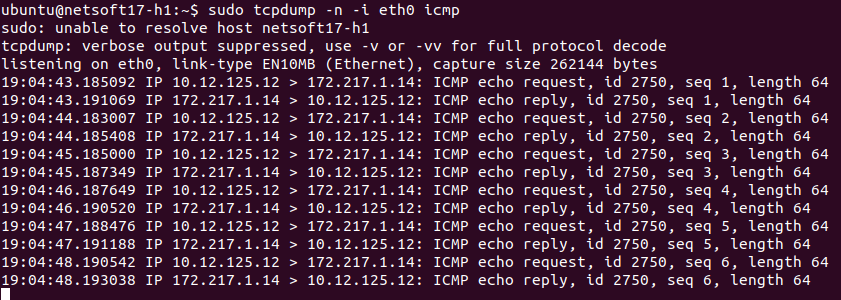
\includegraphics[scale=0.5]{tcpdump-h1}
	\caption{TCP Dump h1}
\end{figure}

\vspace{5mm} 
\textbf{Part 2}

\vspace{2mm} 
\textit{include screenshots clearly showing the correctness of your implementation: 
	a routing table from either h2 or h3, and the relevant iptables entry for
	turning h1 into a NAT router}
\vspace{2mm} 

\begin{figure}[h]
	\centering
	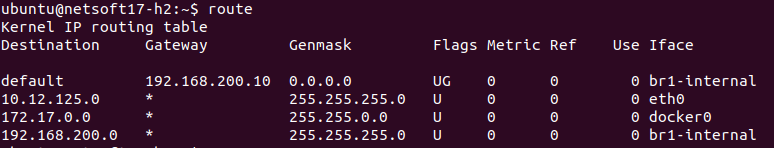
\includegraphics[scale=0.5]{h2-route-table}
	\caption{h2 routing table}
\end{figure}

\begin{figure}[h]
	\centering
	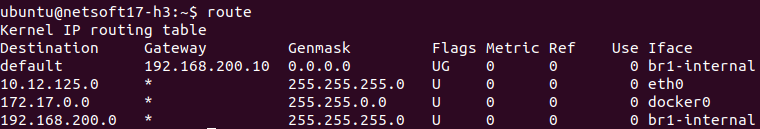
\includegraphics[scale=0.5]{h3-route-table}
	\caption{h3 routing table}
\end{figure}


\begin{minted}{text}
sudo iptables -t nat -A POSTROUTING -o eth0 -j MASQUERADE
sudo iptables -P FORWARD ACCEPT

Chain POSTROUTING (policy ACCEPT)
target     prot opt source               destination
MASQUERADE  all  --  172.17.0.0/16        anywhere
MASQUERADE  all  --  anywhere             anywhere
\end{minted}

\begin{minted}{text}
ubuntu@netsoft17-h2:~$ route
Kernel IP routing table
Destination     Gateway         Genmask         Flags Metric Ref    Use Iface
default         192.168.200.10  0.0.0.0         UG    0      0        0 br1-internal
10.12.125.0     *               255.255.255.0   U     0      0        0 eth0
172.17.0.0      *               255.255.0.0     U     0      0        0 docker0
192.168.200.0   *               255.255.255.0   U     0      0        0 br1-internal
\end{minted}

\begin{minted}{text}
ubuntu@netsoft17-h3:~$ route
Kernel IP routing table
Destination     Gateway         Genmask         Flags Metric Ref    Use Iface
default         192.168.200.10  0.0.0.0         UG    0      0        0 br1-internal
10.12.125.0     *               255.255.255.0   U     0      0        0 eth0
172.17.0.0      *               255.255.0.0     U     0      0        0 docker0
192.168.200.0   *               255.255.255.0   U     0      0        0 br1-internal
\end{minted}


\vspace{5mm} 
\textbf{Part 3.3}

\begin{minted}{text}
in_port={port num of vxlan iface},priority={something high},dl_dst={mac
	of internal iface created by saviOverlay},actions=output:{port num of
internal iface created by saviOverlay}
\end{minted}

This rule redirects any traffic related to the internal interface to the internal
internal interface.

\begin{minted}{text}
in_port={port num of vxlan iface},priority={something
high},dl_dst=01:00:00:00:00:00/01:00:00:00:00:00,actions=output:{
port num of internal iface created by saviOverlay }
\end{minted}

This rule redirects any broadcast traffic related to the internal interface to the internal interface.

\begin{minted}{text}
in_port={port num of internal iface created by saviOverlay},actions=output:{port num of vxlan iface}
\end{minted}

This rule redirects any traffic from the internal interface to the vxlan interface
to be delivered to other switches. This traffic is any traffic other than the
traffic which was directed using SDN rules installed later on. The higher priority
is because it is not required for other traffics to be passed inside the snort.


\begin{minted}{text}
in_port={port num of vxlan iface},priority={something lower than
before},actions=output:{port num of snort ingress iface}
\end{minted}

This rule redirects any traffic not related to internal interface to the
snort ingress port. This is basically the traffic which was directed using SDN
and is actually destinted for h3. The lower priority is used because we don't
want to interere with a traffic which was not destined for h3.

\begin{minted}{text}
in_port={port num of vxlan iface},priority={something lower than
before},actions=output:{port num of snort ingress iface}
\end{minted}

\begin{minted}{text}
in_port={port num of snort egress iface},priority={something lower than
before},actions=output:{port num of vxlan iface}
\end{minted}
This rule redirects any traffic coming out of the snort ingress port
to be delivered to the destination.


\begin{minted}{text}
ubuntu@imant-h3:~$ sudo ovs-ofctl show br1
sudo: unable to resolve host imant-h3
OFPT_FEATURES_REPLY (xid=0x2): dpid:0000164b6e819f44
n_tables:254, n_buffers:256
capabilities: FLOW_STATS TABLE_STATS PORT_STATS QUEUE_STATS ARP_MATCH_IP
actions: output enqueue set_vlan_vid set_vlan_pcp strip_vlan mod_dl_src mod_dl_dst mod_nw_src mod_nw_dst mod_nw_tos mod_tp_src mod_tp_dst
 1(br1-internal): addr:0a:ca:8a:da:ec:a4
     config:     0
     state:      0
     speed: 0 Mbps now, 0 Mbps max
 2(imant-h3-imant-): addr:16:96:3d:4d:aa:74
     config:     0
     state:      0
     speed: 0 Mbps now, 0 Mbps max
 3(snort-1): addr:72:7a:eb:72:6c:11
     config:     PORT_DOWN
     state:      LINK_DOWN
     speed: 0 Mbps now, 0 Mbps max
 4(snort-2): addr:86:97:05:2d:3f:c4
     config:     PORT_DOWN
     state:      LINK_DOWN
     speed: 0 Mbps now, 0 Mbps max
 LOCAL(br1): addr:16:4b:6e:81:9f:44
     config:     PORT_DOWN
     state:      LINK_DOWN
     speed: 0 Mbps now, 0 Mbps max
OFPT_GET_CONFIG_REPLY (xid=0x4): frags=normal miss_send_len=0
\end{minted}

\begin{minted}{text}
ubuntu@imant-h3:~$ sudo ovs-ofctl dump-flows br1
sudo: unable to resolve host imant-h3
NXST_FLOW reply (xid=0x4):
 cookie=0x0, duration=140.013s, table=0, n_packets=443, n_bytes=39886, idle_age=0, priority=60000,in_port=2,dl_dst=0a:ca:8a:da:ec:a4 actions=output:1
 cookie=0x0, duration=127.489s, table=0, n_packets=140, n_bytes=7140, idle_age=1, priority=60000,in_port=2,dl_dst=01:00:00:00:00:00/01:00:00:00:00:00 actions=output:1
 cookie=0x0, duration=117.099s, table=0, n_packets=182, n_bytes=20356, idle_age=0, in_port=1 actions=output:2
 cookie=0x0, duration=105.494s, table=0, n_packets=0, n_bytes=0, idle_age=105, priority=50000,in_port=2 actions=output:3
 cookie=0x0, duration=94.100s, table=0, n_packets=0, n_bytes=0, idle_age=94, priority=50000,in_port=4 actions=output:2
 cookie=0x0, duration=20585.874s, table=0, n_packets=25253, n_bytes=1406768, idle_age=117, priority=0 actions=NORMAL

\end{minted}


\vspace{2mm} 
\textit{inport}
\vspace{2mm} 

\textbf{Part 3.4}

\vspace{2mm} 
\textit{reject tcp any any -> any 80 (content:"inject"; nocase; msg:"accessed forbidden pages!!"; sid:5000000;)}
\vspace{2mm} 

The first of the rule tells the action to be applied to the matching rule in 
this case \textit{reject}. The second word tells which protocol does this 
rule apply to. In this case the protocol is \textit{ip}. The third word 
tells what is the source ip address. In this case source ip address 
is \textit{any}. The fourth word specifies the source port number. 
In this case source port number is \textit{any}. The part after arrow specifies 
the destination specification. Also, the direction of the arrow indicates the 
direction of interest. The first word after arrow is destination ip address 
which in this case is \textit{any}. The second word
after arrow is the destination port number which in this case is \textit{80}.
The part in the paranthesis specifies the specific options regarding the rule. 
The \textit{nocase} option is used to deactivate any case sensitivity in the 
content rule. The \textit{msg} specifies the message to be printed along the 
packet dump. The \textit{sid} is used for specifying a particular snort rule.
This can be used by external plugins to identify snort rules.


\vspace{5mm} 
\textbf{Part 4.4}

\vspace{2mm} 

You can find the code for installing flows in the appendix section. Unfortunately,
because my VMs were deleted (3 times), I didn't find enough time to go through
the lab again from the beginning. This is the reason why flow dumps are missing
from this section.

\begin{minted}{text}
ubuntu@imant-sw3:~$ sudo ovs-ofctl dump-flows br1
sudo: unable to resolve host imant-sw3
NXST_FLOW reply (xid=0x4):
 cookie=0x0, duration=21387.397s, table=0, n_packets=23729, n_bytes=1210179, idle_age=1, priority=65535,dl_dst=01:80:c2:00:00:0e,dl_type=0x88cc actions=CONTROLLER:51
 cookie=0x0, duration=79.049s, table=0, n_packets=30, n_bytes=6274, idle_age=45, priority=60000,tcp,in_port=1,dl_src=76:eb:89:2e:25:70,dl_dst=5a:b5:e9:15:cc:ec,tp_dst=80 actions=output:2
 cookie=0x0, duration=24.857s, table=0, n_packets=0, n_bytes=0, idle_timeout=60, hard_timeout=60, idle_age=24, in_port=2,dl_src=0a:ca:8a:da:ec:a4,dl_dst=ff:ff:ff:ff:ff:ff actions=FLOOD
 cookie=0x0, duration=24.803s, table=0, n_packets=0, n_bytes=0, idle_timeout=60, hard_timeout=60, idle_age=24, in_port=1,dl_src=76:eb:89:2e:25:70,dl_dst=0a:ca:8a:da:ec:a4 actions=output:2
\end{minted}

\begin{minted}{text}
sudo: unable to resolve host imant-sw1
NXST_FLOW reply (xid=0x4):
 cookie=0x0, duration=21433.695s, table=0, n_packets=47572, n_bytes=2426172, idle_age=0, priority=65535,dl_dst=01:80:c2:00:00:0e,dl_type=0x88cc actions=CONTROLLER:51
 cookie=0x0, duration=3249.019s, table=0, n_packets=0, n_bytes=0, idle_age=3249, priority=60000,tcp,in_port=1,dl_src=3a:43:e9:0c:a2:d0,dl_dst=d6:cd:3d:01:c9:ec,tp_dst=80 actions=output:2
 cookie=0x0, duration=3249.018s, table=0, n_packets=0, n_bytes=0, idle_age=3249, priority=60000,tcp,in_port=2,dl_src=3a:43:e9:0c:a2:d0,dl_dst=d6:cd:3d:01:c9:ec,tp_dst=80 actions=output:3
 cookie=0x0, duration=130.100s, table=0, n_packets=30, n_bytes=6274, idle_age=96, priority=60000,tcp,in_port=1,dl_src=76:eb:89:2e:25:70,dl_dst=5a:b5:e9:15:cc:ec,tp_dst=80 actions=output:2
 cookie=0x0, duration=130.099s, table=0, n_packets=30, n_bytes=3829, idle_age=96, priority=60000,tcp,in_port=2,dl_src=76:eb:89:2e:25:70,dl_dst=5a:b5:e9:15:cc:ec,tp_dst=80 actions=output:3
\end{minted}


\textbf{Part 4.5}

\vspace{2mm} 


\begin{figure}[h]
	\centering
	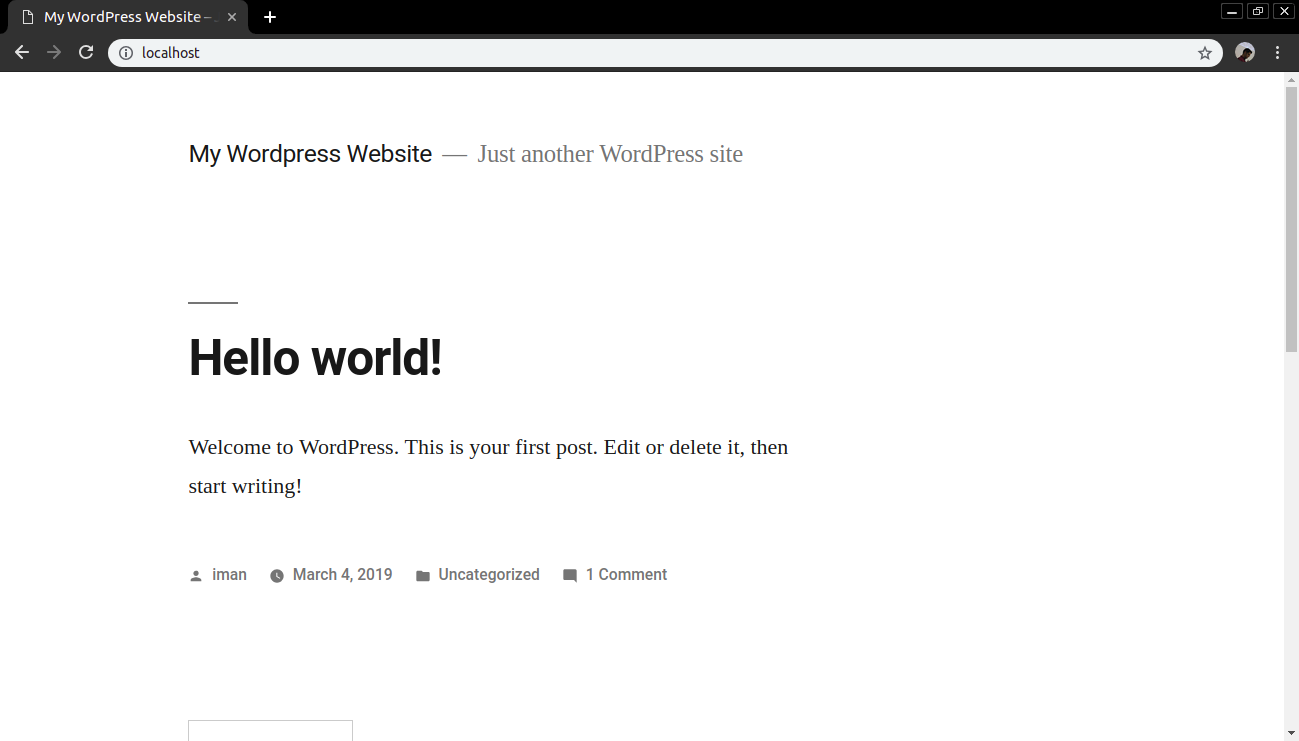
\includegraphics[scale=0.3]{working}
	\caption{Loading WordPress}
\end{figure}

\begin{figure}[h]
	\centering
	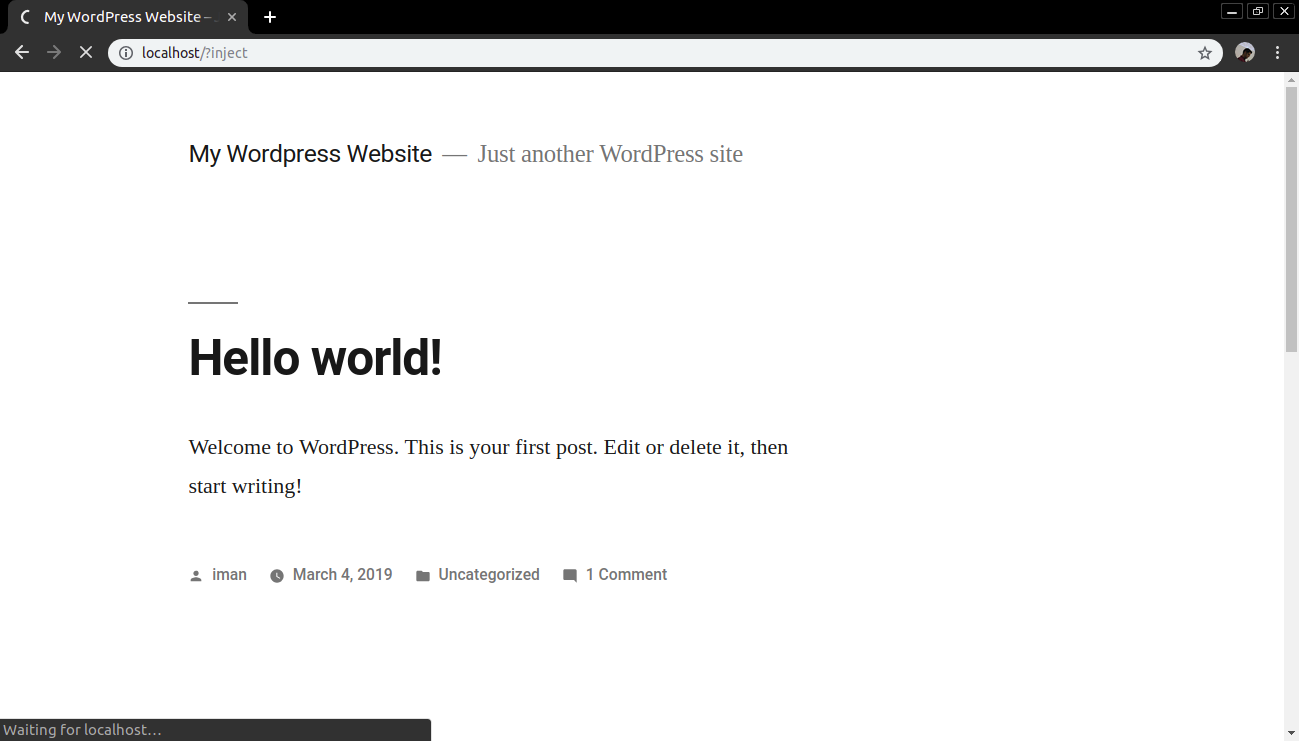
\includegraphics[scale=0.3]{not-loading}
	\caption{Not Loading WordPress if we use inject}
\end{figure}

\begin{figure}[h]
	\centering
	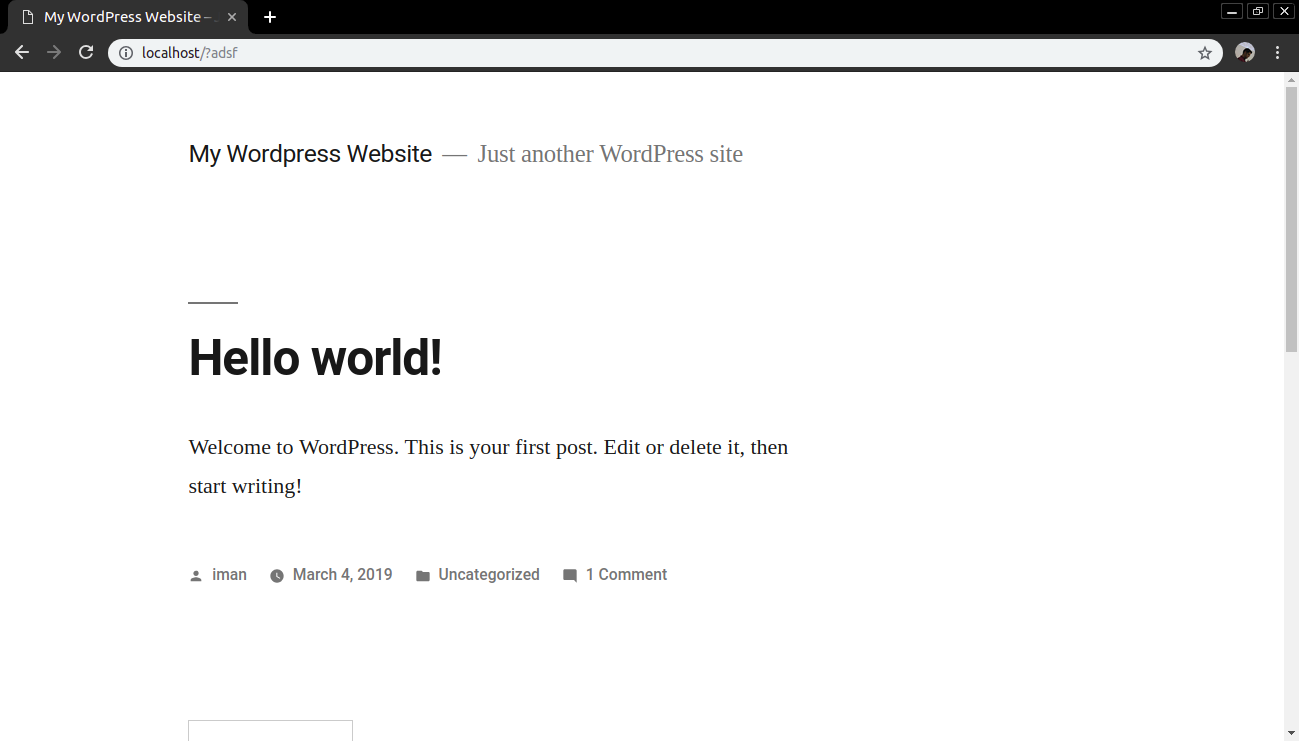
\includegraphics[scale=0.3]{other-endpoint-working}
	\caption{Other endpoints working}
\end{figure}

\begin{figure}[h]
	\centering
	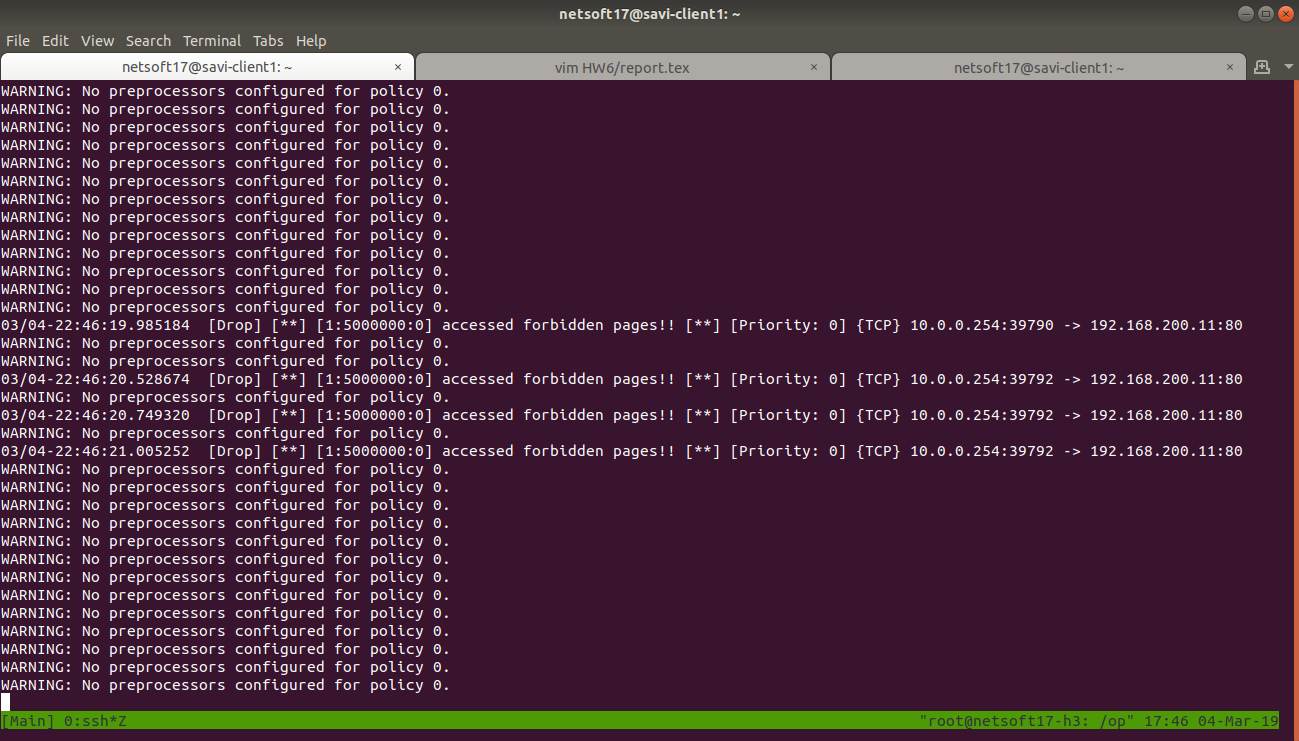
\includegraphics[scale=0.3]{snort-blocking}
	\caption{Snort logs showing blocking of connection}
\end{figure}

\clearpage

\textbf{Appendix}

\begin{minted}{python}

import ryu_ofctl

h2 = "5a:b5:e9:15:cc:ec"
h3 = "0a:ca:8a:da:ec:a4"
h1 = "76:eb:89:2e:25:70"

sw1 = '00002a38cb041745'
sw2 = "0000e601655db64f"
sw3 = "0000fa9ecd0fb541"


sw1_flows = [
    ryu_ofctl.FlowEntry(),
    ryu_ofctl.FlowEntry(),
    ryu_ofctl.FlowEntry()
]

# Flow 1 (h1 -> h3 for initial inspection) (sw1)
sw1_flows[0].dl_src = h1
sw1_flows[0].dl_dst = h2
sw1_flows[0].in_port = 1
sw1_flows[0].dl_type = 0x800
sw1_flows[0].nw_proto = 0x6
sw1_flows[0].tp_dst = 80
sw1_flows[0].priority = 60000
sw1_flows[0].addAction(ryu_ofctl.OutputAction(2))
ryu_ofctl.insertFlow(sw1, sw1_flows[0])

# Flow 2 (h3 -> h2 for passing after processing) (sw1)
sw1_flows[1].dl_src = h1
sw1_flows[1].dl_dst = h2
sw1_flows[1].in_port = 2
sw1_flows[1].dl_type = 0x800
sw1_flows[1].nw_proto = 0x6
sw1_flows[1].tp_dst = 80
sw1_flows[1].priority = 60000
sw1_flows[1].addAction(ryu_ofctl.OutputAction(3))
ryu_ofctl.insertFlow(sw1, sw1_flows[1])

# Flow 3 (h3 -> h2 for passing after processing) (sw3)
sw1_flows[2].dl_src = h1
sw1_flows[2].dl_dst = h2
sw1_flows[2].in_port = 1
sw1_flows[2].dl_type = 0x800
sw1_flows[2].nw_proto = 0x6
sw1_flows[2].tp_dst = 80
sw1_flows[2].priority = 60000
sw1_flows[2].addAction(ryu_ofctl.OutputAction(2))
ryu_ofctl.insertFlow(sw3, sw1_flows[2])
\end{minted}
\end{document}
